\documentclass[10pt]{beamer}

\usetheme[progressbar=frametitle]{metropolis}
\usepackage{appendixnumberbeamer}
\usepackage[compat=1.0.0]{tikz-feynman}
\usepackage[]{biblatex}
\addbibresource{resources.bib}

\definecolor{c1}{rgb}{1,0.93,0.8}


\title{Building SUSY models II: using superfields}
\subtitle{Seminar on Supersymmetry and its breaking}
\author{Matteo Zortea}
\date{Universit\"at Heidelberg, $27^{th}$ May 2022}
\institute{Coordinated by prof. Joerg Jaeckel}

\makeatletter
\setbeamertemplate{title page}{
  \begin{minipage}[b][\paperheight]{\textwidth}
    \centering  % <-- Center here
    \ifx\inserttitlegraphic\@empty\else\usebeamertemplate*{title graphic}\fi
    \vfill%
    \ifx\inserttitle\@empty\else\usebeamertemplate*{title}\fi
    \ifx\insertsubtitle\@empty\else\usebeamertemplate*{subtitle}\fi
    \usebeamertemplate*{title separator}
    \ifx\beamer@shortauthor\@empty\else\usebeamertemplate*{author}\fi
    \ifx\insertdate\@empty\else\usebeamertemplate*{date}\fi
    \ifx\insertinstitute\@empty\else\usebeamertemplate*{institute}\fi
    \vfill
    \vspace*{1mm}
  \end{minipage}
}

\setbeamertemplate{title}{
%  \raggedright%  % <-- Comment here
  \linespread{1.0}%
  \inserttitle%
  \par%
  \vspace*{0.5em}
}
\setbeamertemplate{subtitle}{
%  \raggedright%  % <-- Comment here
  \insertsubtitle%
  \par%
  \vspace*{0.5em}
}
\makeatother




\begin{document}

\begin{frame}
\titlepage
\end{frame}

\begin{frame}{Main points of the talk}
\begin{itemize}
    \item Apply the superspace formalism and show why it is useful to build SUSY theories
    \item Principles to construct SUSY lagrangians 
    \item Feynman diagrams for supersymmetric theories
    \item SUSY gauge theories: QED and QCD
    \item SUSY predictions: particles, superparticles, interactions, ...
\end{itemize}
$\rightarrow$ Search for a lagrangian that under a SUSY transformation
\begin{equation*}
    \mathcal{L} \to \mathcal{L} + \partial_\mu f
\end{equation*}
\end{frame}

\begin{frame}{How to build SUSY invariant lagrangians}
    \begin{itemize} 
        \item Left-chiral field expansion (right-chiral is hermitian conjugate)
            \begin{gather*}
                \Phi(x, \theta, \bar\theta) = \varphi(x) + i\bar\theta \bar\sigma^{\mu}\theta \partial_{\mu}\varphi(x) + \frac{1}{4}\theta\theta\bar\theta\bar\theta\partial_{\mu}\partial^{\mu}\varphi(x) + \sqrt{2}\theta\psi(x) + \\ 
                -\frac{i}{\sqrt{2}}\theta\theta\bar\theta\bar\sigma^{\mu}\partial_{\mu}\psi(x) + \theta\theta F(x)
            \end{gather*}
        \item Vector field expansion
            \begin{gather*}
                V\left(x, \theta, \bar\theta\right) = a+\theta \xi+\bar\theta \xi^{\dagger} +\theta \theta b+\bar\theta \bar\theta b^{\dagger}+\bar\theta \bar{\sigma}^{\mu} \theta A_{\mu}+ \\ 
                + \bar\theta \bar\theta \theta\left(\lambda-\frac{i}{2} \sigma^{\mu} \partial_{\mu} \xi^{\dagger}\right)
                +\theta \theta \bar\theta\left(\lambda^{\dagger}-\frac{i}{2} \sigma^{\mu} \partial_{\mu} \xi\right)+\theta \theta \bar\theta \bar\theta \left(\frac{1}{2} D+\frac{1}{4} \partial_{\mu} \partial^{\mu} a\right)
            \end{gather*}
        \item They both carry no spinor, nor vector indices, the name is due to their particle content! 
    \end{itemize}
\end{frame}

\begin{frame}{How to build SUSY invariant lagrangians}
\begin{itemize}
    \item For the components of a chiral field $\Phi(x, \theta, \bar\theta)$ one has that
        \begin{gather*}
                \delta_{\epsilon} \phi =\epsilon \psi \\
                \delta_{\epsilon} \psi_{\alpha} =-i\left(\sigma^{\mu} \epsilon^{\dagger}\right)_{\alpha} \partial_{\mu} \phi+\epsilon_{\alpha} F, \\
                \boxed{\delta_{\epsilon} F =-i \epsilon^{\dagger} \bar{\sigma}^{\mu} \partial_{\mu} \psi}
        \end{gather*}
    \item For the components of a vector field $V(x, \theta, \bar\theta)$ one has
        \begin{gather*}
                \sqrt{2} \delta_{\epsilon} a =\epsilon \xi+\epsilon^{\dagger} \xi^{\dagger} \qquad 
                \sqrt{2} \delta_{\epsilon} \lambda_{\alpha} =\epsilon_{a} D+\frac{i}{2}\left(\sigma^{\mu} \sigma^{\nu} \epsilon\right)_{\alpha}\left(\partial_{\mu} A_{\nu}-\partial_{\nu} A_{\mu}\right) \\
                \sqrt{2} \delta_{\epsilon} b =\epsilon^{\dagger} \lambda^{\dagger}-i \epsilon^{\dagger} \sigma^{\mu} \partial_{\mu} \xi \qquad
                \sqrt{2} \delta_{\epsilon} \xi_{\alpha} =2 \epsilon_{\alpha} b-\left(\sigma^{\mu} \epsilon^{\dagger}\right)_{\alpha}\left(A_{\mu}+i \partial_{\mu} a\right) \\
                \sqrt{2} \delta_{\epsilon} A^{\mu} =i \epsilon \partial^{\mu} \xi-i \epsilon^{\dagger} \partial^{\mu} \xi^{\dagger}+\epsilon \sigma^{\mu} \lambda^{\dagger}-\epsilon^{\dagger} \bar{\sigma}^{\mu} \lambda \\
                \boxed{\sqrt{2} \delta_{\epsilon} D =-i \epsilon \sigma^{\mu} \partial_{\mu} \lambda^{\dagger}-i \epsilon^{\dagger} \bar{\sigma}^{\mu} \partial_{\mu} \lambda}
        \end{gather*}
\end{itemize}
\end{frame}

\begin{frame}{How to build SUSY invariant lagrangians}
\begin{itemize}
    \item Idea $\rightarrow$ "select" the components of the fields that transforms as total derivatives
    \item How can we "pick" only the terms we need? $\rightarrow$ Grassman integration
    \begin{gather*}
        \int d^2\theta \quad \theta^n \, f(x, \bar\theta) \ = \ f(x, \bar\theta) \, \delta_{n, 2} \\
        \int d^2\theta d^2\bar\theta \quad \bar\theta^m \theta^n \, f(x)  \ = \ f(x) \, \delta_{m, 2} \, \delta_{n, 2}
    \end{gather*}
    \item Our terms of interest
    \begin{gather*}
        \left[\Phi\right]_F = \int d^2\theta \ \Phi(x, \theta, \bar\theta) = F + \text{total derivative} \\
        \left[V\right]_D = \int d^2\theta d^2\bar\theta \ V(x, \theta, \bar\theta) = \frac{1}{2} \, D + \text{total derivative}
    \end{gather*}
\end{itemize}
\end{frame}

\begin{frame}{How to build SUSY invariant lagrangians}
    Let us focus for a moment on the D term.
    \begin{gather*}
        \Phi(x, \theta, \bar\theta) = \varphi(x) + i\bar\theta \bar\sigma^{\mu}\theta \partial_{\mu}\varphi(x) + \frac{1}{4}\theta\theta\bar\theta\bar\theta\partial_{\mu}\partial^{\mu}\varphi(x) + \sqrt{2}\theta\psi(x)\\ 
        -\frac{i}{\sqrt{2}}\theta\theta\bar\theta\bar\sigma^{\mu}\partial_{\mu}\psi(x) + \theta\theta F(x) \\
        \Phi^{\dagger i} \Phi_{j}= \varphi^{* i} \varphi_{j}+\sqrt{2} \theta \psi_{j} \varphi^{* i}+\sqrt{2} \bar\theta \psi^{\dagger i} \varphi_{j}+\theta \theta \varphi^{* i} F_{j}+\bar\theta \bar\theta \varphi_{j} F^{\dagger i} \\
            +\bar\theta \bar{\sigma}^{\mu} \theta\left[i \varphi^{* i} \partial_{\mu} \varphi_{j}-i \varphi_{j} \partial_{\mu} \varphi^{* i}-\psi^{\dagger i} \sigma_{\mu} \psi_{j}\right] \\
                +\frac{i}{\sqrt{2}} \theta \theta \bar\theta \bar{\sigma}^{\mu}\left(\psi_{j} \partial_{\mu} \varphi^{* i}-\partial_{\mu} \psi_{j} \varphi^{* i}\right)+\sqrt{2} \theta \theta \bar\theta \psi^{\dagger i} F_{j} \\
                +\frac{i}{\sqrt{2}} \bar\theta \bar\theta \theta \sigma^{\mu}\left(\psi^{\dagger i} \partial_{\mu} \varphi_{j}-\partial_{\mu} \psi^{\dagger i} \varphi_{j}\right)+\sqrt{2} \bar\theta \bar\theta \theta \psi_{j} F^{* i} \\
                +\theta \theta \bar\theta \bar\theta\left[F^{* i} F_{j}-\frac{1}{2} \partial^{\mu} \varphi^{* i} \partial_{\mu} \varphi_{j}+\frac{1}{4} \varphi^{* i} \partial^{\mu} \partial_{\mu} \varphi_{j}+\frac{1}{4} \varphi_{j} \partial^{\mu} \partial_{\mu} \varphi^{* i}\right. \\
                \left.+\frac{i}{2} \psi^{\dagger i} \bar{\sigma}^{\mu} \partial_{\mu} \psi_{j}+\frac{i}{2} \psi_{j} \sigma^{\mu} \partial_{\mu} \psi^{\dagger i}\right]
    \end{gather*}
    One can note that for $i=j$ one has that $(\Phi^{\dagger}\Phi)^{\dagger} = \Phi^{\dagger}\Phi \Rightarrow$ vector field!
\end{frame}
\begin{frame}{How to build SUSY invariant lagrangians}
    \begin{itemize}[<+->]
        \item Now "select" the SUSY invariant component (D component)
        \begin{gather*}
            \left[\Phi^{\dagger}\Phi\right]_D = \int d^2\theta d^2\bar\theta \ \Phi^{\dagger}(x, \theta, \bar\theta) \Phi(x, \theta, \bar\theta) \\
            \left[F^{*} F - \frac{1}{2} \partial^{\mu} \varphi^{*} \partial_{\mu} \varphi+\frac{1}{4} \varphi^{*} \partial^{\mu} \partial_{\mu} \varphi+\frac{1}{4} \varphi \partial^{\mu} \partial_{\mu} \varphi^{*}\right. \\
                    \left.+\frac{i}{2} \psi^{\dagger} \bar{\sigma}^{\mu} \partial_{\mu} \psi+\frac{i}{2} \psi \sigma^{\mu} \partial_{\mu} \psi^{\dagger}\right] = \\
            = -\partial^{\mu}\varphi^*\partial_{\mu}\varphi + i\psi^{\dagger}\bar\sigma^{\mu}\partial_{\mu}\psi + F^{*}F + \text{total derivative}
        \end{gather*}
        \item Hence 
        \begin{equation*}
            \boxed{S = \int dx^{\mu} \mathcal{L} = \int dx^{\mu} \left( -\partial^{\mu}\varphi^{*}\partial_{\mu}\varphi + i\psi^{\dagger}\bar\sigma^{\mu}\partial_{\mu}\psi + F^{*}F \right)}
        \end{equation*}
        \centerline{\bfseries $\rightarrow$ Free Wess-Zumino model!}
    \end{itemize}
\end{frame}

\begin{frame}{How to build SUSY invariant lagrangians}
    \begin{itemize}
        \item In order to add SUSY invariant interactions, let us recall the definitions of chiral superfields 
            \begin{equation*}
                \bar D_{\dot\alpha} \Phi = 0 \qquad D_{\alpha} \Phi^{\dagger} = 0
            \end{equation*}
        \item Note that any analytic function of chiral superfields is in turn a chiral superfield (power series expansion and product rule). \\
        \item $\Rightarrow$ Write our chiral term of $N$ fields as 
            \begin{equation*}
                W(\{\Phi_k\}) = \sum_i^N a_i \Phi_i + \sum_{i,j}^N \frac{1}{2!} m_{ij} \Phi_{i}\Phi_j + \sum_{i,j,k}^N \frac{1}{3!} y_{ijk} \Phi_i \Phi_j \Phi_k
            \end{equation*}
        \item Higher order terms are non-renormalisable \\
        \item Reality of the action requires us to take $W + W^*$
        \item $W$ is called \emph{superpotential}
    \end{itemize}
\end{frame}

\begin{frame}{How to buld SUSY invariant lagrangians}
The interacting lagrangian becomes
\begin{gather*}
\mathcal{L}_{WZ}\left(\{\Phi_i\}, \{\Phi^{\dagger}_i\}\right) = \mathcal{L}_{WZ,D} + \mathcal{L}_{WZ,F} = \\
= \left[\Phi^{\dagger i}\Phi^i\right]_D + \left[W(\{\Phi_i\})\right]_F +  \left[W^{\dagger}(\{\Phi^{\dagger}_i\})\right]_F = \\
= \int d^2\theta \ \left(-\frac{1}{4}\overline{DD}\Phi^{\dagger i}\Phi_i + W(\{\Phi_i\})\right) + \int d^2\bar\theta \ W^{\dagger}(\{\Phi^{\dagger}_i\}) = \\
= \int d^2\bar\theta \ \left(-\frac{1}{4}{DD}\Phi^{\dagger i}\Phi_i + W(\{\Phi_i\})\right) + \int d^2\bar\theta \ W^{\dagger}(\{\Phi^{\dagger}_i\})
\end{gather*}
where I used that 
\begin{equation*}
    \int d^2\theta d^2\bar\theta \Phi^{\dagger}\Phi = - \int d^2\theta \, \frac{1}{4} \, \overline{DD}\Phi^\dagger\Phi = - \int d^2\bar\theta \, \frac{1}{4} \, DD(\Phi^{\dagger}\Phi) 
\end{equation*}
Equations of motion varying w.r.t. $\Phi_i$ and $\Phi_i^{\dagger}$
\begin{gather*}
    0=-\frac{1}{4} \overline{D D} \Phi^{\dagger i}+\frac{\delta W}{\delta \Phi_{i}} \qquad
    0=-\frac{1}{4} D D \Phi_{i}+\frac{\delta W^{\dagger}}{\delta \Phi^{\dagger i}}
\end{gather*}
\end{frame}

\begin{frame}{Wess-Zumino model}
    \begin{itemize}
        \item We are now interested in studying better the components of $\Phi$, hence let us focus on the case $i=j$ with $a_{i} = a, m_{ij}=m, y_{ijk}=y$ and the superpotential
            \begin{equation*}
                W(\Phi) = \frac{1}{2} \, m \, \Phi\Phi + \frac{1}{3!} \,  y \, \Phi \Phi \Phi
            \end{equation*}
            where we dropped the linear term.
        \item The lagrangian becomes
            \begin{gather*}
                \mathcal{L}(\Phi, \Phi^{\dagger}) = \mathcal{L}_{WZ, D} + \mathcal{L}_{WZ, F} = \\ 
                = F^{*} F+\left(\partial_{\mu} \varphi\right)\left(\partial^{\mu} \varphi\right)^{*}+\frac{i}{2} \psi \sigma^{\mu}\left(\partial_{\mu} \psi^{\dagger}\right)-\frac{i}{2}\left(\partial_{\mu} \psi\right) \sigma^{\mu} \psi^{\dagger} + \\
                    -m \varphi F-\frac{m}{2}(\psi \psi)-\frac{y}{2} \varphi \varphi F-\frac{y}{2} \varphi(\psi \psi)+\text { h.c. }
            \end{gather*}
        \item E.o.m. for $F$ (analogous for $F^{*}$) is
            \begin{gather*}
                0=\partial_{\mu} \frac{\partial \mathcal{L}}{\partial\left(\partial_{\mu} F\right)}-\frac{\partial \mathcal{L}}{\partial F}=-\frac{\partial \mathcal{L}}{\partial F}=-F^{*}+m \varphi+\frac{y}{2} \varphi \varphi
            \end{gather*}
        \item $\Rightarrow$ algebraic equation $\Rightarrow$ $F,F^{*}$ are unphysical. 
    \end{itemize}
\end{frame}

\begin{frame}{Wess-Zumino model}
    \begin{equation*}
        F^{*} = m\varphi + \frac{y}{2}\varphi\varphi \qquad F = m \varphi^{*} + \frac{y}{2} \varphi \varphi
    \end{equation*}
    \begin{itemize}
        \item One can rewrite the terms containing $F, F^{*}$ as  
        \begin{equation*}
            F^{*} F-\left(m \varphi F+\frac{y}{2} \varphi \varphi F+h c\right)=-\left|m \varphi+\frac{y}{2} \varphi \varphi\right|^{2}=-\left|\frac{\partial W(\varphi)}{\partial \varphi}\right|^{2}
        \end{equation*}
        that is, the superpotential evaluated at the scalar field value $F = \varphi$!
        \item The lagrangian then becomes
        \begin{equation*}
            \begin{aligned}
                \mathcal{L}_{\mathrm{Wz}} &=\left(\partial_{\mu} \varphi\right)\left(\partial^{\mu} \varphi\right)^{\dagger}+\frac{i}{2} \psi \sigma^{\mu}\left(\partial_{\mu} \psi^{\dagger}\right)-\frac{i}{2}\left(\partial_{\mu} \psi\right) \sigma^{\mu} \psi^{\dagger} \\
                &-|M|^{2} \varphi \varphi^*-\frac{|y|^{2}}{4} \varphi \varphi \varphi^* \varphi^* \\
                &- \left(\frac{M}{2} \psi \psi+\frac{M \cdot y}{2} \varphi \varphi \varphi^*+\frac{y}{2} \varphi \psi \psi+\text { h.c. }\right)
                \end{aligned}
        \end{equation*}
        
        %    and one can prove that in the case of $N$ fields it can be written as 
        %    \begin{equation*}
        %    \begin{aligned}
        %        \mathcal{L}_{W Z} &=\left(\partial_{\mu} \varphi_{i}\right)\left(\partial^{\mu} \varphi_{i}\right)^{\dagger}+\frac{i}{2} \psi_{i} \sigma^{\mu}\left(\partial_{\mu} \psi^{\dagger}_{i}\right)-\frac{i}{2}\left(\partial_{\mu} \psi_{i}\right) \sigma^{\mu} \psi^{\dagger}_{i} \\
        %        &-\sum_{i}\left|\frac{\partial W\left(\varphi_{i}\right)}{\partial \varphi_{i}}\right|^{2}-\frac{1}{2}\left(\frac{\partial^{2} W\left(\varphi_{i}\right)}{\partial \varphi_{i} \partial \varphi_{j}}\right) \psi_{i} \psi_{j}-\frac{1}{2}\left(\frac{\partial^{2} W^{\dagger}\left(\varphi_{i}\right)}{\partial \varphi_{i}^{\dagger} \partial \varphi_{j}^{\dagger}}\right) \psi^{\dagger}_{i} \psi^{\dagger}_{j}
        %        \end{aligned}
        %    \end{equation*}
        \end{itemize}
\end{frame}

\begin{frame}{Wess-Zumino model}
    The lagrangian can also be written as
    \begin{equation*}
        \begin{aligned}
            \mathcal{L}_{\mathrm{Wz}} &=\left(\partial_{\mu} \varphi\right)\left(\partial^{\mu} \varphi\right)^{\dagger}+\frac{i}{2} \psi \sigma^{\mu}\left(\partial_{\mu} \psi^{\dagger}\right)-\frac{i}{2}\left(\partial_{\mu} \psi\right) \sigma^{\mu} \psi^{\dagger} \\
            &-|M|^{2} \varphi \varphi^*-\frac{|y|^{2}}{4} \varphi \varphi \varphi^* \varphi^*-\left(\frac{M}{2} \psi \psi+\frac{M \cdot y}{2} \varphi \varphi \varphi^*+\frac{y}{2} \varphi \psi \psi+\text { h.c. }\right) \\
            &=\left(\partial_{\mu} \varphi\right)\left(\partial^{\mu} \varphi\right)^{*}+\frac{i}{2} \psi \sigma^{\mu}\left(\partial_{\mu} \psi^{\dagger}\right)-\frac{i}{2}\left(\partial_{\mu} \psi\right) \sigma^{\mu} \psi^{\dagger} \\
            &-\left|\frac{\partial W\left(\varphi\right)}{\partial \varphi}\right|^{2}-\frac{1}{2}\left(\frac{\partial^{2} W\left(\varphi\right)}{\partial \varphi \partial \varphi}\right) \psi \psi-\frac{1}{2}\left(\frac{\partial^{2} W^{*}\left(\varphi\right)}{\partial \varphi^{*} \partial \varphi^{*}}\right) \psi^{\dagger} \psi^{\dagger}
        \end{aligned}
    \end{equation*}
    where, I remember,
    \begin{equation*}
        W(\Phi) = \frac{1}{2} \, M \, \Phi\Phi + \frac{1}{3!} \, y \, \Phi\Phi\Phi
    \end{equation*}
\end{frame}

\begin{frame}{Wess-Zumino model}
    \begin{equation*}
        \begin{aligned}
            \mathcal{L}_{\mathrm{Wz}} &=\left(\partial_{\mu} \varphi\right)\left(\partial^{\mu} \varphi\right)^{*}+\frac{i}{2} \psi \sigma^{\mu}\left(\partial_{\mu} \psi^{\dagger}\right)-\frac{i}{2}\left(\partial_{\mu} \psi\right) \sigma^{\mu} \psi^{\dagger} \\
            &-|M|^{2} \varphi \varphi^{*}-\frac{|y|^{2}}{4} \varphi \varphi \varphi^{*} \varphi^{*}-\left(\frac{M}{2} \psi \psi+\frac{M \cdot y}{2} \varphi \varphi \varphi^{*}+\frac{y}{2} \varphi \psi \psi+\text { h.c. }\right)
            \end{aligned}
    \end{equation*}
    Let us give a look at the interactions (diagrams taken from \cite{MARTIN_1998})
        \begin{figure}
            \centering
            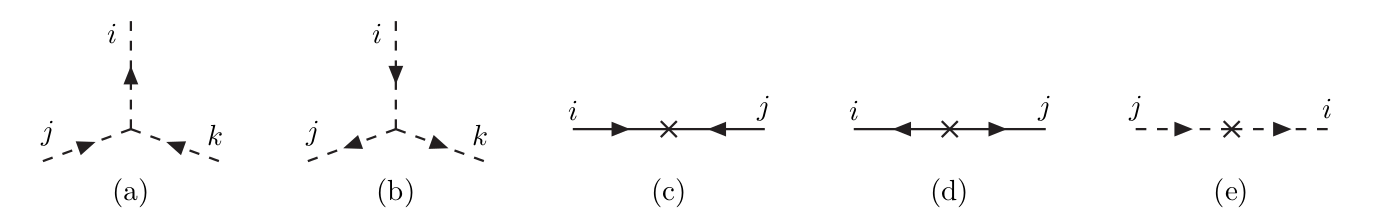
\includegraphics[scale=0.22]{feynman1.png}
            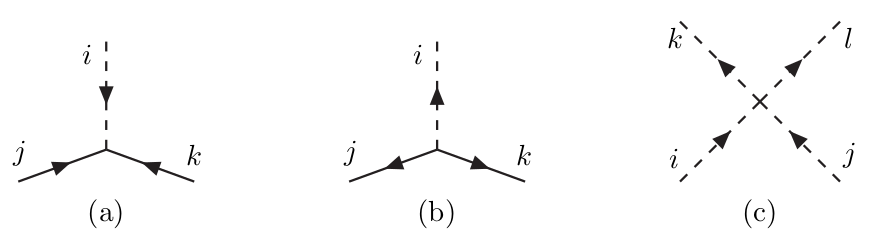
\includegraphics[scale=0.22]{feynman2.png}
        \end{figure}
\end{frame}

\begin{frame}{Nonrenormalization theorem}
    One can check straighforwardly that the quadratic divergence in the boson's mass is cancelled! \\
    One can prove that in general the following theorem holds \\ 
    \vspace{15pt}
    \fbox{\begin{minipage}{0.8\textwidth}\emph{The superpotential is not renormalised at any order in perturbation theory. Thus it might get affected by nonperturbative effects such as instantons}\end{minipage}}
    \\
    \vspace*{15pt}
    This is the so called \textbf{N=1 nonrenormalization theorem}
\end{frame}
    
\begin{frame}{Abelian gauge theories}
Let us now introduce (abelian) gauge interactions
\begin{itemize} 
    \item Let us start with U(1) global symmetry 
    \begin{equation*}
        \Phi_i \rightarrow e^{iq_i\Lambda_i}\Phi_i
    \end{equation*}
    \item The kinetic part of the lagrangian is always invariant
    \begin{equation*}
        \mathcal{L}_{K} = \mathcal{L}_{WZ,D} = \int d^2\theta d^2 \bar\theta \ \Phi^{\dagger}\Phi = \int d^2\theta -\frac{1}{4} \overline{D D} \Phi^{\dagger}\Phi
    \end{equation*}
    \item The interaction part 
    \begin{equation*}
        \mathcal{L}_{int} = \mathcal{L}_{WZ,F} = \int d^2\theta \ \frac{1}{2} \sum_{ij} \, m_{ij} \, \Phi_i \Phi_j + \frac{1}{3!} \sum_{ijk}  \, y_{ijk} \, \Phi_i \Phi_j \Phi_k + \text{h.c.}
    \end{equation*}
    requires
    \begin{equation*}
        m_{ij} = 0 \qquad \text{or} \qquad y_{ijk} = 0
    \end{equation*}
    whenever
    \begin{equation*}
        q_i + q_j \neq 0 \qquad \text{or} \qquad q_i + q_j + q_k \neq 0
    \end{equation*}
\end{itemize}
\end{frame}

\begin{frame}{Abelian gauge theories}
Promote to a local gauge symmetry
\begin{equation*}
    \Lambda \to \Lambda(x, \theta, \bar\theta)
\end{equation*}
\begin{itemize}
    \item The gauge parameter is now a supergauge field $\Lambda = \Lambda(x, \theta, \bar\theta)$
    \item We need $\Lambda(x, \theta, \bar\theta)$ to be a left-chiral superfield if we want $\Phi'$ to be a left-chiral superfield. \\ 
    \item Thus this causes a problem in the kinetic term because $\Lambda^{\dagger}$ is a right-chiral superfield
    hence obviously $\Phi'^{\dagger}\Phi' \neq \Phi^{\dagger}\Phi$
    \item The problem is analogous to the kinetc term in "normal" QFT when $\partial_u \varphi^* \partial^\mu \varphi$ was not gauge invariant
    \item Solution: add a term that compensate the gauge for the non invariant terms
\end{itemize}
\end{frame}

\begin{frame}{Abelian gauge theories}
Recall from the previous talk that a gauge transformation on a vector field $V$ reads
\begin{equation*}
    V \to V' = V + i(\Lambda^{\dagger} - \Lambda)
\end{equation*}
one can modify the kinetic term to
\begin{equation*}
    \Phi^{\dagger} e^V \Phi
\end{equation*}
so that it is invariant under the above gauge transformations
\begin{equation*}
    \Phi^{\dagger}e^V\Phi \to \Phi '^{\dagger}  e^{V'} \Phi ' = \Phi^{\dagger}e^{-i\Lambda^{\dagger}}e^{i\Lambda*}e^Ve^{-i\Lambda}e^{i\Lambda}\Phi = \Phi^{\dagger}e^V\Phi
\end{equation*}

\end{frame}


\begin{frame}{Abelian gauge theories}
Let us now define the two chiral fields \\
\begin{equation*}
    \mathcal{W}_{\alpha}=-\frac{1}{4} \overline{D D} D_{\alpha} V, \quad \overline{\mathcal{W}}_{\dot{\alpha}} = -\frac{1}{4} D D \bar{D}_{\dot{\alpha}} V
\end{equation*}
where $V$ is a vector field. \\
The gauge-invariant dynamical term (equivalent to $F_{\mu\nu} F^{\mu\nu}$) is 
\begin{equation*}
   [\mathcal{W}\mathcal{W}]_F + [\overline{\mathcal{W}\mathcal{W}}]_F = \int d^2\theta \ \mathcal{W}_{\alpha} \mathcal{W}^{\alpha} + \int d^2\bar\theta \ \overline{\mathcal{W}}_{\dot\alpha} \overline{\mathcal{W}}^{\dot\alpha}
\end{equation*}
The explicit derivation is quite long but we can make two checks to get more convinced
\begin{itemize}
    \item Check that it is indeed gauge invariant
    \item Check that it contains the "normal" gauge strength field $F_{\mu\nu}F^{\mu\nu}$ after integrating out $\theta$ and $\bar\theta$
\end{itemize}
\end{frame}

\begin{frame}{Abelian gauge theories}
To see that it is gauge invariant remember that under a $U(1)$ transformation $V \to V + i\left(\Omega^{\dagger} - \Omega\right)$ and that 
$D_\alpha \Omega = 0, \bar D^{\dot \alpha} \Omega = 0$
\begin{equation*}
\begin{aligned}
    \mathcal{W}_{\alpha} \rightarrow-\frac{1}{4} \overline{D D} D_{\alpha}\left[V+i\left(\Omega^{\dagger}-\Omega\right)\right] &=\mathcal{W}_{\alpha}+\frac{i}{4} \overline{D D} D_{\alpha} \Omega \\
    &=\mathcal{W}_{\alpha}-\frac{i}{4} \bar{D}^{\dot{\beta}}\left\{\bar{D}_{\dot{\beta}}, D_{\alpha}\right\} \Omega \\
    &=\mathcal{W}_{\alpha}+\frac{1}{2} \sigma_{\alpha \dot{\beta}}^{\mu} \partial_{\mu} \bar{D}^{\dot{\beta}} \Omega \\
    &=\mathcal{W}_{\alpha}
\end{aligned}
\end{equation*}
where I also used that 
\begin{equation*}
    \left\{\bar{D}_{\bar\beta}, D_{\alpha}\right\}= - 2 i \sigma_{\alpha \dot{\beta}}^{\mu} \partial_{\mu},
\end{equation*}
\end{frame}

\begin{frame}{Abelian gauge theories}
Remember that in the Wess-Zumino gauge the field expansion takes the form 
\begin{gather*}
    V(y, \theta, \bar \theta) = \bar\theta \bar{\sigma}^{\mu} \theta A_{\mu}(y)+\bar\theta \bar\theta \theta \lambda(y)+\theta \theta \bar\theta \lambda^{\dagger}(y) + \\ 
    \frac{1}{2} \theta \theta \theta \bar\theta \bar\theta\left[D(y)+i \theta_{\mu} A^{\mu}(y)\right]
\end{gather*}
Hence 
\begin{equation*}
    \mathcal{W}_{\alpha}\left(y, \theta, \bar\theta\right)=\lambda_{a}+\theta_{\alpha} D+\frac{i}{2}\left(\sigma^{\mu} \bar{\sigma}^{\nu} \theta\right)_{\alpha} F_{\mu \nu}+i \theta \theta\left(\sigma^{\mu} \partial_{\mu} \lambda^{\dagger}\right)_{\alpha}
\end{equation*}
Finally 
\begin{equation*}
    \frac{1}{4}\left[\mathcal{WW}\right]_F + \frac{1}{4} \left[\overline{\mathcal{WW}}\right]_F = -\frac{1}{4} F_{\mu\nu} F^{\mu\nu} + i \lambda^{\dagger} \bar\sigma^{\mu} \partial_{\mu} \lambda + \frac{1}{2} D^2
\end{equation*}
We recovered the desired term $F_{\mu\nu}F^{\mu\nu}$, but what are the other two terms?
\end{frame}

\begin{frame}{Abelian gauge theories}
The term 
\begin{equation*}
    i\lambda^{\dagger} \bar\sigma^{\mu}\partial_{\mu} \lambda
\end{equation*}
is just the superpartner of the photon, the \emph{photino}! \\
For the other term, we can show that it plays no physical role (as the F term in the chiral fields). To do this we need to spot all the $D$ dependence in our lagrangian. \\
Remembering that up to now our lagrangian is 
\begin{equation*}
    \mathcal{L} = \frac{1}{4}\left[\mathcal{WW}\right]_F + \frac{1}{4} \left[\overline{\mathcal{WW}}\right]_F + \left[\Phi^{\dagger} e^V \Phi\right]_D + [W(\Phi)]_F + [\bar W(\Phi^{\dagger})]_F
\end{equation*}
once can note that the only other dependence on D is in $\left[\Phi^{\dagger} e^V \Phi \right]_D = \Phi^{\dagger}\Phi D$.
Hence the equation of motions for $D$ are
\begin{equation*}
    0 = \frac{\partial \mathcal{L}}{\partial D} = D + \Phi^{\dagger} \Phi 
\end{equation*}
\end{frame}

\begin{frame}{Abelian gauge theories}
Putting all together we get the SUSY QED lagrangian 
\begin{gather*}
    \mathcal{L}=\left[\Phi^{* i} e^{q_i V}{\Phi_{i}}\right]_{D}+\left(\left[W\left(\Phi_{i}\right)\right]_{F}+\text { c.c. }\right)+\frac{1}{4}\left(\left[\mathcal{W}^{\alpha} \mathcal{W}_{\alpha}\right]_{F}+\text { c.c. }\right)
\end{gather*}
To this we add another SUSY and supergauge invariant term $2[kV]_D = 2kD$ (e.o.m. is still algebraic). 
This term is called \emph{Fayet-Iliopoulos} and it will play an important role in the spontaneous SUSY breaking (next talks)
\begin{equation*}
    \boxed{
        \begin{gathered}
        \mathcal{L}_{SQED} = \left[\Phi^{* i} e^{q_{i} V} {\Phi_{i}}\right]_{D}+\left(\left[W\left(\Phi_{i}\right)\right]_{F}+\text { c.c. }\right)+ \\ 
        +\frac{1}{4}\left(\left[\mathcal{W}^{\alpha} \mathcal{W}_{\alpha}\right]_{F}+\text { c.c. }\right)-2 \kappa[V]_{D}
        \end{gathered}}
\end{equation*}
\end{frame}

\begin{frame}{Non abelian gauge theories}
Now extend to generic gauge theories, in particular SU(n). In spacetime:
\begin{itemize}
    \item $n^2-1$ generators $T_{1}, \dots T_{n^2-1}$ (gauge fields)
    \item for $n=3$ we have 8 fields (gluons)
    \item $\left[T_a, T_b\right] = i \, f_{abc} \, T_c$ where $f_{abc}$ are called structure constants
    \item $U \in SU(n) \Rightarrow U = \exp(i g A^a T^a)$
    \item Covariant derivatives  in spacetime are $D_\mu = \partial_\mu - ig A_\mu = \partial_\mu - igA_u^a T^a$
\end{itemize}
In spacetime, guided by the fact that for $U(1)$ we had $$F_{\mu\nu} = \partial_\mu A_\nu - \partial_\nu A_\mu = \frac{i}{e} \, [D_\mu, D_\nu]$$
we \emph{define} our field strength tensor for a general gauge symmetry via 
\begin{equation*} 
    F_{\mu \nu} \equiv \frac{i}{g} \, [D_\mu, D_\nu] = \partial_\mu A_\nu - \partial_\nu A_\mu -ig \, [A_\mu, A_\nu]
\end{equation*}
In superspace proceed analogously by "generalising" the definition
\end{frame}

\begin{frame}{Non abelian gauge theories}
    We note that 
    \begin{equation*} 
        e^V \to e^{V + i(\Lambda^\dagger - \Lambda)}
    \end{equation*}
    Is a particular case of 
    \begin{equation*}
        e^V \to e^{i\Lambda^\dagger} e^V e^{-i\Lambda}
    \end{equation*}
    when the commutators vanish $[\Lambda^\dagger, V] = 0 = [\Lambda, V]$. \\
    In fact
    \begin{align*}
        V \rightarrow V &+ i\left(\Omega^{\dagger}-\Omega\right)-\frac{i}{2}\left[V, \Omega+\Omega^{\dagger}\right] + \\ 
        &+ i \sum_{k=1}^{\infty} \frac{B_{2 k}}{(2 k) !}\left[V,\left[V, \ldots\left[V, \Omega^{\dagger}-\Omega\right] \ldots\right]\right] = \\
        = &+ i\left(\Omega^{a *}-\Omega^{a}\right)+g_{a} f^{a b c} V^{b}\left(\Omega^{c *}+\Omega^{c}\right) \\ 
        &-\frac{i}{3} g_{a}^{2} f^{a b c} f^{c d^{b}} V^{b} V^{d}\left(\Omega^{c}-\Omega^{r}\right)+\ldots
    \end{align*}
    where $B_n$ defined by $\frac{x}{e^{x}-1}=\sum_{n=0}^{\infty} \frac{B_{n}}{n !} x^{n}$ are the Bernoulli numbers
\end{frame}

\begin{frame}{Non abelian gauge theories}
We have to generalise also the kinetic term 
\begin{equation*}
    \mathcal{W}_{\alpha}=-\frac{1}{4} \overline{D D}\left(e^{-V} D_{\alpha} e^{V}\right)
\end{equation*}
so that it is invariant under 
\begin{equation*}
    \mathcal{W}_{\alpha} \rightarrow e^{i \Omega} \mathcal{W}_{\alpha} e^{-i \Omega}
\end{equation*}
The lagrangian then becomes 
\begin{equation*}
    \mathcal{L}=\frac{1}{4}\left[\mathcal{W}^{a \alpha} W_{\alpha}^{a}\right]_{F}+c . c .+\left[\Phi^{*i}\left(e^{2 g_a T^{a} V^{a}}\right)_{i}^j \Phi_{j}\right]_{D}+\left(\left[W\left(\Phi_{i}\right)\right]_F+c . c .\right) .
\end{equation*}
Let us write it in components in the case of SU(3) (QCD) after eliminating $F,D$ via e.o.m.
\end{frame}

\begin{frame}{NSQCD interactions}
In case of QCD
\begin{equation*}
    \begin{aligned}
        \mathcal{L} &=\left(D_{\mu} \varphi_{i}\right)^{*}\left(D^{\mu} \varphi\right)_{i}+\frac{i}{2} \psi_{i} \sigma^{\mu}\left(D_{\mu} \psi^{\dagger}\right)_{i}-\frac{i}{2}\left(D_{\mu} \psi\right)_{i} \sigma^{\mu} \psi^{\dagger}_{i}\\
        &-\frac{1}{4} F_{\mu \nu}^{a}\left(F^{a}\right)^{\mu \nu}+\frac{i}{2} \lambda^{a} \sigma^{\mu}\left(D_{\mu} \bar{\lambda}\right)^{a}-\frac{i}{2}\left(D_{\mu} \lambda\right)^{a} \sigma^{\mu} \bar{\lambda}^{a} \\
        &-\sqrt{2} i g \psi^{\dagger}_{i} \bar{\lambda}^{a} T_{i j}^{a} \varphi_{j}+\sqrt{2 i g} \varphi_{i}^{\dagger} T_{i j}^{a} \psi_{j} \lambda^{a} \\
        &-\frac{1}{2} \frac{\partial^{2} W}{\partial \varphi_{i} \partial \varphi_{j}} \psi_{i} \psi_{j}-\frac{1}{2} \frac{\partial^{2} W^{\dagger}}{\partial \varphi_{i}^{*} \partial \varphi_{j}^{*}} \psi^{\dagger}_{i} \psi^{\dagger}_{j}-V\left(\varphi_{i}, \varphi_{j}^{*}\right)
        \end{aligned}
\end{equation*}
where 
\begin{equation*}
    V\left(\varphi_{i}, \varphi_{j}^{*}\right)=F_{i}^{*} F_{i}+\frac{1}{2}\left(D^{a}\right)^{2}=\sum_{i}\left|\frac{\partial W}{\partial \varphi_{i}}\right|^{2}+\frac{1}{2} \sum_{a}\left(g \varphi_{i}^{*} T_{i j}^{a} \varphi_{j}+k^{a}\right)^{2}
\end{equation*}
\begin{equation*}
    W\left(\varphi_{i}\right)=a_{i} \varphi_{i}+\frac{1}{2} m_{i j} \varphi_{i} \varphi_{j}+\frac{1}{3 !} y_{i j k} \varphi_{i} \varphi_{j} \varphi_{k}
\end{equation*}
\end{frame}

\begin{frame}{SQCD interactions}
    Where the gauge covariant derivatives are
    \begin{equation*}\begin{aligned}
        \left(D_{\mu} \varphi\right)_{i} &=\partial_{\mu} \varphi_{i}+i g v_{\mu}^{a} T_{i j}^{a} \varphi_{j} \\
        \left(D_{\mu} \psi\right)_{i} &=\partial_{\mu} \psi_{i}+i g v_{\mu}^{a} T_{i j}^{a} \psi_{j} \\
        \left(D_{\mu} \lambda\right)^{a} &=\partial_{\mu} \lambda^{a}-g f^{a b c} v_{\mu}^{b} \lambda^{c}
        \end{aligned}
    \end{equation*}
\end{frame}

\begin{frame}{SQCD interactions}
    This gives very cool interactions (diagrams from \cite{Signer_2009})
    \begin{figure}
        \centering 
        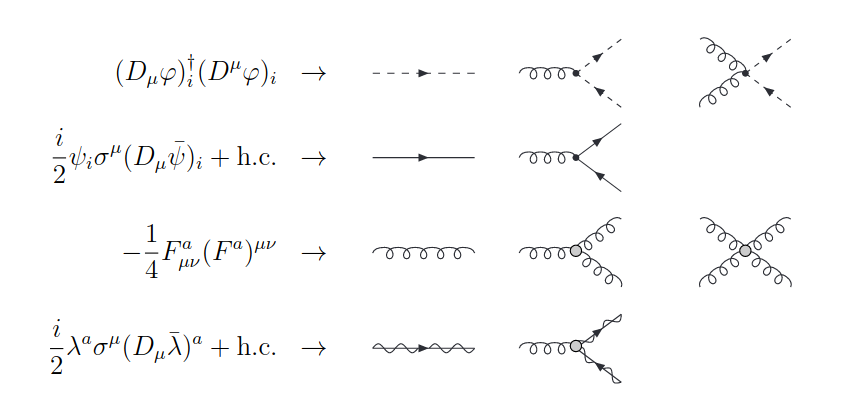
\includegraphics[scale=0.35]{sqcd_inter_2.png}
    \end{figure}
\end{frame}

\begin{frame}{SQCD interactions}
    \pagenumbering{gobble}
    \begin{figure}
        \centering 
        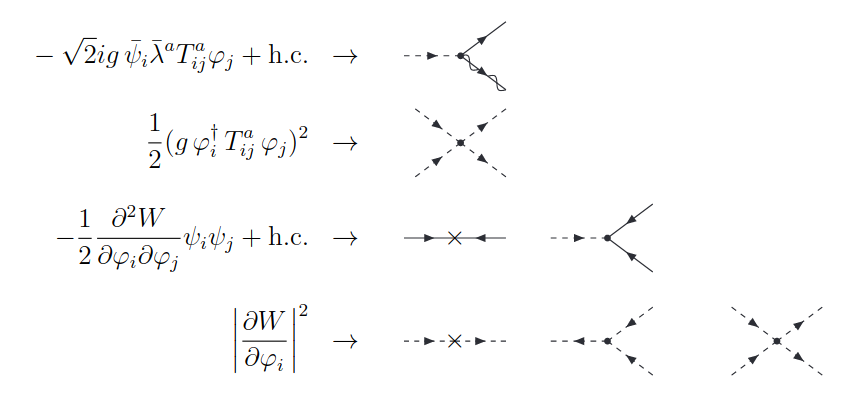
\includegraphics[scale=0.35]{sqcd_inter_1.png}
    \end{figure}
\end{frame}


{
\setbeamercolor{background canvas}{bg=c1}
\begin{frame}
    \vfill
    \centerline{Thank you for your attention}
    \vfill
\end{frame}
}

\begin{frame}
    \nocite{*}
    \printbibliography
\end{frame}
\end{document}